\begin{frame}{Sentence Embedding}

\begin{columns}[T]
  \begin{column}{0.40\textwidth}
    \begin{itemize}
        \item Used \textbf{all-MiniLM-L6-v2} sentence transformer
        \item Embedding captures semantic meaning of:
          \begin{itemize}
            \item Title
            \item Authors
            \item Description
          \end{itemize}
        \item Input format for embedding:
          \scriptsize
          \begin{quote}
          Title: ... Author: ... Description: ...
          \end{quote}
        \item 384 dimension embedding vector
        \item Same embedding model used for:
          \begin{itemize}
            \item Book metadata
            \item User query
          \end{itemize}
        \item Enables \textbf{semantic similarity search}, beyond keywords.
    \end{itemize}
  \end{column}

  \begin{column}{0.55\textwidth}
    \centering
    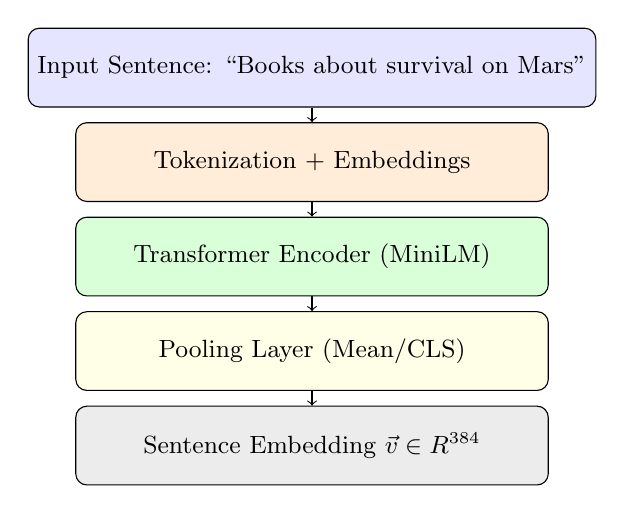
\begin{tikzpicture}[node distance=1.2cm, every node/.style={font=\small}]
        \node (input) [draw, rounded corners, minimum width=6cm, minimum height=1cm, fill=blue!10] {Input Sentence: ``Books about survival on Mars''};

        \node (tokens) [below of=input, draw, rounded corners, minimum width=6cm, minimum height=1cm, fill=orange!15] {Tokenization + Embeddings};

        \node (transformer) [below of=tokens, draw, rounded corners, minimum width=6cm, minimum height=1cm, fill=green!15] {Transformer Encoder (MiniLM)};

        \node (pooling) [below of=transformer, draw, rounded corners, minimum width=6cm, minimum height=1cm, fill=yellow!10] {Pooling Layer (Mean/CLS)};

        \node (vector) [below of=pooling, draw, rounded corners, minimum width=6cm, minimum height=1cm, fill=gray!15] {Sentence Embedding \( \vec{v} \in \mathbb{R}^{384} \)};

        \draw[->] (input) -- (tokens);
        \draw[->] (tokens) -- (transformer);
        \draw[->] (transformer) -- (pooling);
        \draw[->] (pooling) -- (vector);
    \end{tikzpicture}
  \end{column}
\end{columns}

\end{frame}
